\documentclass[aspectratio=169,12pt,t]{beamer}
\usepackage{graphicx}
\setbeameroption{hide notes}
\setbeamertemplate{note page}[plain]
\usepackage{listings}

% header.tex: boring LaTeX/Beamer details + macros

% get rid of junk
\usetheme{default}
\beamertemplatenavigationsymbolsempty
\hypersetup{pdfpagemode=UseNone} % don't show bookmarks on initial view


% font
\usepackage{fontspec}
\setsansfont
  [ ExternalLocation = ../fonts/ ,
    UprightFont = *-regular ,
    BoldFont = *-bold ,
    ItalicFont = *-italic ,
    BoldItalicFont = *-bolditalic ]{texgyreheros}
\setbeamerfont{note page}{family*=pplx,size=\footnotesize} % Palatino for notes
% "TeX Gyre Heros can be used as a replacement for Helvetica"
% I've placed them in fonts/; alternatively you can install them
% permanently on your system as follows:
%     Download http://www.gust.org.pl/projects/e-foundry/tex-gyre/heros/qhv2.004otf.zip
%     In Unix, unzip it into ~/.fonts
%     In Mac, unzip it, double-click the .otf files, and install using "FontBook"

% named colors
\definecolor{offwhite}{RGB}{255,250,240}
\definecolor{gray}{RGB}{155,155,155}
\definecolor{purple}{RGB}{177,13,201}
\definecolor{green}{RGB}{46,204,64}

\definecolor{background}{RGB}{255,255,255}
\definecolor{foreground}{RGB}{24,24,24}
\definecolor{title}{RGB}{27,94,134}
\definecolor{subtitle}{RGB}{22,175,124}
\definecolor{hilit}{RGB}{122,0,128}
\definecolor{vhilit}{RGB}{255,0,128}
\definecolor{codehilit}{RGB}{255,0,128}
\definecolor{lolit}{RGB}{95,95,95}
\definecolor{myyellow}{rgb}{1,1,0.7}
\definecolor{nhilit}{RGB}{128,0,128}  % hilit color in notes
\definecolor{nvhilit}{RGB}{255,0,128} % vhilit for notes

\newcommand{\hilit}{\color{hilit}}
\newcommand{\vhilit}{\color{vhilit}}
\newcommand{\nhilit}{\color{nhilit}}
\newcommand{\nvhilit}{\color{nvhilit}}
\newcommand{\lolit}{\color{lolit}}

% use those colors
\setbeamercolor{titlelike}{fg=title}
\setbeamercolor{subtitle}{fg=subtitle}
\setbeamercolor{institute}{fg=lolit}
\setbeamercolor{normal text}{fg=foreground,bg=background}
\setbeamercolor{item}{fg=foreground} % color of bullets
\setbeamercolor{subitem}{fg=lolit}
\setbeamercolor{itemize/enumerate subbody}{fg=lolit}
\setbeamertemplate{itemize subitem}{{\textendash}}
\setbeamerfont{itemize/enumerate subbody}{size=\footnotesize}
\setbeamerfont{itemize/enumerate subitem}{size=\footnotesize}

% page number
\setbeamertemplate{footline}{%
    \raisebox{5pt}{\makebox[\paperwidth]{\hfill\makebox[20pt]{\lolit
          \scriptsize\insertframenumber}}}\hspace*{5pt}}

% add a bit of space at the top of the notes page
\addtobeamertemplate{note page}{\setlength{\parskip}{12pt}}

% default link color
\hypersetup{colorlinks, urlcolor={hilit}}

\lstset{language=bash,
        basicstyle=\ttfamily\scriptsize,
        frame=single,
        commentstyle=,
        backgroundcolor=\color{offwhite},
        showspaces=false,
        showstringspaces=false
        }


% a few macros
\newcommand{\bi}{\begin{itemize}}
\newcommand{\bbi}{\vspace{24pt} \begin{itemize} \itemsep8pt}
\newcommand{\ei}{\end{itemize}}
\newcommand{\be}{\begin{enumerate}}
\newcommand{\bbe}{\vspace{24pt} \begin{enumerate} \itemsep8pt}
\newcommand{\ee}{\end{enumerate}}
\newcommand{\ig}{\includegraphics}
\newcommand{\subt}[1]{{\footnotesize \color{subtitle} {#1}}}
\newcommand{\ttsm}{\tt \small}
\newcommand{\ttfn}{\tt \footnotesize}
\newcommand{\figh}[2]{\centerline{\includegraphics[height=#2\textheight]{#1}}}
\newcommand{\figw}[2]{\centerline{\includegraphics[width=#2\textwidth]{#1}}}


%%%%%%%%%%%%%%%%%%%%%%%%%%%%%%%%%%%%%%%%%%%%%%%%%%%%%%%%%%%%%%%%%%%%%%
% end of header
%%%%%%%%%%%%%%%%%%%%%%%%%%%%%%%%%%%%%%%%%%%%%%%%%%%%%%%%%%%%%%%%%%%%%%

\title{Wrangling messy data files}
\author{\href{https://kbroman.org}{Karl Broman}}
\institute{Biostatistics \& Medical Informatics, UW{\textendash}Madison}
\date{\href{https://kbroman.org}{\tt \scriptsize \color{foreground} kbroman.org}
\\[-4pt]
\href{https://github.com/kbroman}{\tt \scriptsize \color{foreground} github.com/kbroman}
\\[-4pt]
\href{https://twitter.com/kwbroman}{\tt \scriptsize \color{foreground} @kwbroman}
\\[-4pt]
{\scriptsize Course web: \href{https://kbroman.org/AdvData}{\tt kbroman.org/AdvData}}
}

\begin{document}

{
\setbeamertemplate{footline}{} % no page number here
\frame{
  \titlepage

\note{
  In this lecture, we'll look at the problem of wrangling messy data
  files: A bit of data diagnostics, but mostly how to reorganize data
  files.
}
} }


\begin{frame}[c]{}

\centering
\Large

{
\color{title}

``In what form would you like the data?''
}

\bigskip \bigskip

\onslide<2->{
{\hilit

    ``In its present form!''
}
}

\bigskip \bigskip \bigskip \bigskip
\onslide<3>{
\lolit
\large
\qquad \qquad \qquad   ...so we'll have some messy files to deal with.
}

\note{
  When collaborators ask me how I would like them to send me data, I
  always say: in its present form.

  I cannot emphasize enough: If any transformation needs to be
  done, or if anything needs to be fixed, it is the data scientist who
  is in the best position to do the work, reproducibly and without
  introducing further errors.

  But that means I spend a lot of time mucking about with some pretty
  messy files.  In the lecture today, I want to impart some tips on
  things I've learned, doing so.
}

\end{frame}


\begin{frame}{Challenges}

  \bigskip

  {\large \vhilit Consistency}

  \bigskip

  \bi
\item file names
\item file organization
\item subject IDs
\item variable names
\item categorical data
  \ei

    \note{
      Essentially all of the challenges come from inconsistencies: in
      file names, the arrangement of data within files, the subject
      identifiers, the variable names, and the categories in
      categorical data.

      Code re-organizing data is the worst code.
    }

\end{frame}



\begin{frame}[c]{Example file}

  \figw{Figs/pheno_data.png}{1.0}

  \note{
    Here's an example file. Lots of work was done to prettify things,
    which means multiple header rows and a good amount of work to
    identify and pull out the essential columns.
  }
\end{frame}


\begin{frame}[c]{Another example}

  \figw{Figs/necropsy_data.png}{1.0}

  \note{
    Here's a second worksheet from that file. Again, the header row
    has information on multiple lines that need to be merged. With the
    merged cells, it's hard to predict where they end up in a CSV file.

    The format of individual identifiers is constantly changing.
  }
\end{frame}


\begin{frame}{Weird rounding}

    \figw{Figs/weird_rounding.png}{1.0}

\note{
  Part of that file shows some weird rounding patterns. The font isn't
  even consistent. This suggests to me that there has been some
  copy-pasting of data, and that there may be some other set of files
  that is the primary source for the data.
}
\end{frame}


\begin{frame}{Inconsistent IDs}

  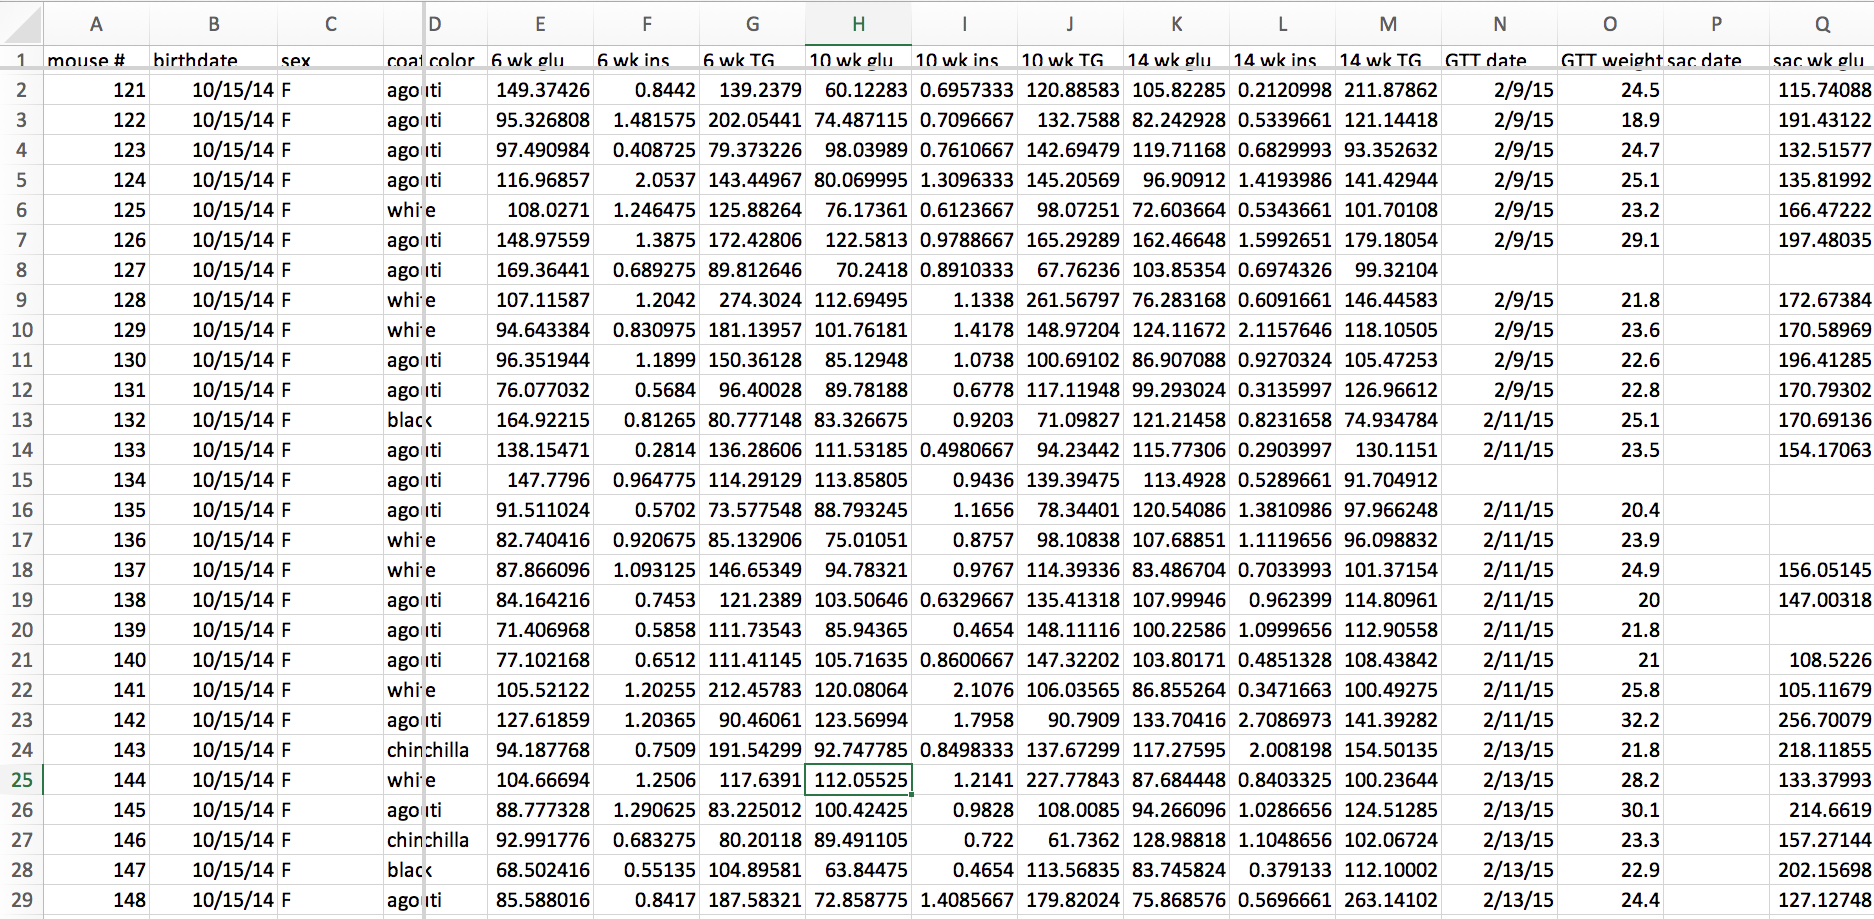
\includegraphics[width=0.8\textwidth]{Figs/attiedo_wave2_sheet1.png}

  \only<2>{
    \vspace{-0.5\textheight}
    \hspace{0.1\textwidth}
    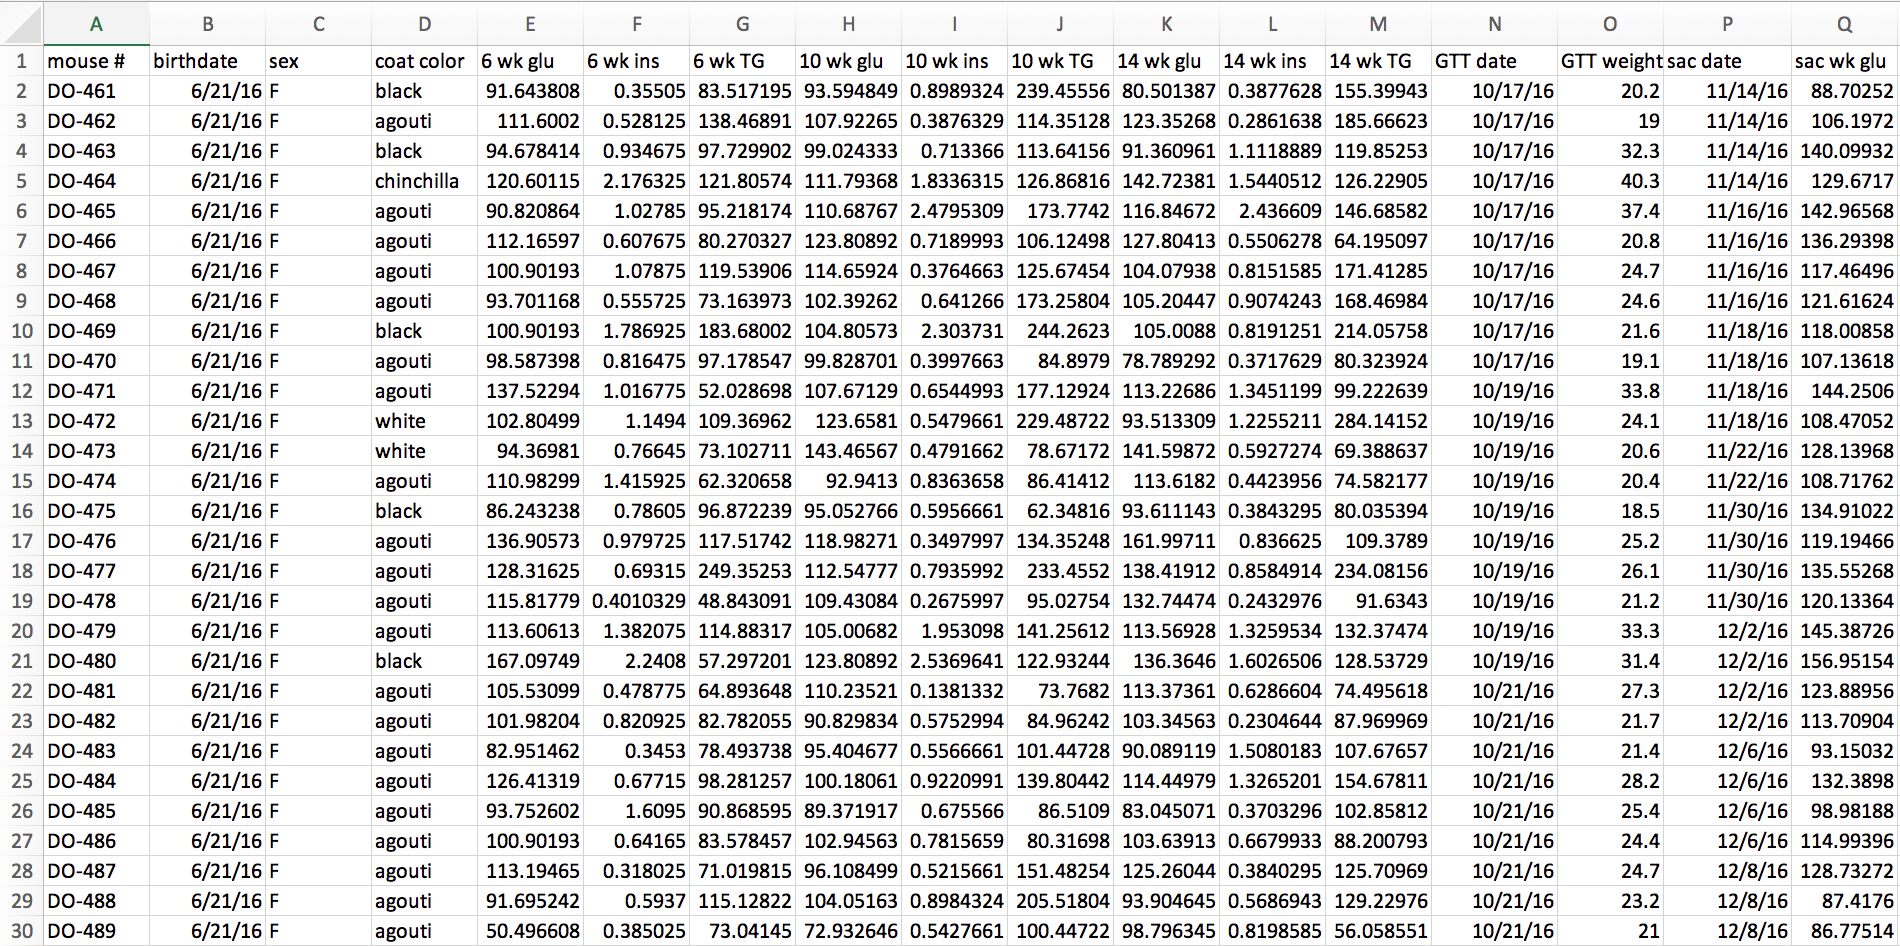
\includegraphics[width=0.8\textwidth]{Figs/attiedo_wave5_sheet1.png}
  }

\note{
  The format of the IDs is different between these files. Also in one
  of the files, there are missing dates that will need to be grabbed
  from some separate file.
}
\end{frame}





\begin{frame}[c]{Inconsistent layout}

  \begin{columns}
    \column{0.5\textwidth}

    \figw{Figs/attiedo_wave2_gtt.png}{1.0}

    \column{0.5\textwidth}

    \figh{Figs/attiedo_wave3_gtt.png}{0.8}
  \end{columns}


\note{
  Another example of inconsistent layout. And messy, in both cases.
  You need to fill in the repeated values like mouse ID, and the
  column names are missing in the file on the right.
}
\end{frame}


\begin{frame}{All kinds of inconsistencies}

  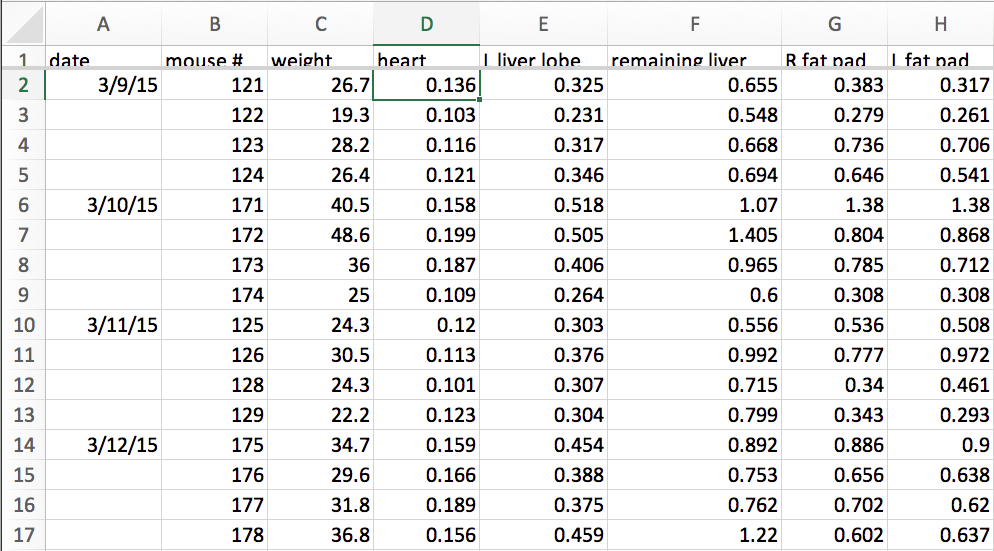
\includegraphics[height=0.6\textheight]{Figs/attiedo_wave2_sacwts.png}

  \only<2->{
    \vspace{-0.5\textheight}
    \hspace{0.1\textwidth}
  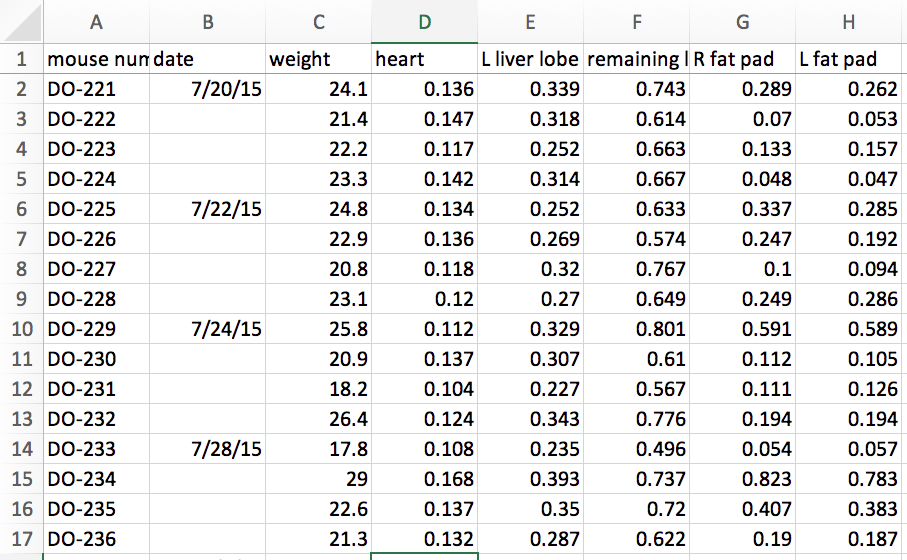
\includegraphics[height=0.6\textheight]{Figs/attiedo_wave3_sacwts.png}
  }

  \only<3->{
    \vspace{-0.5\textheight}
    \hspace{0.2\textwidth}
  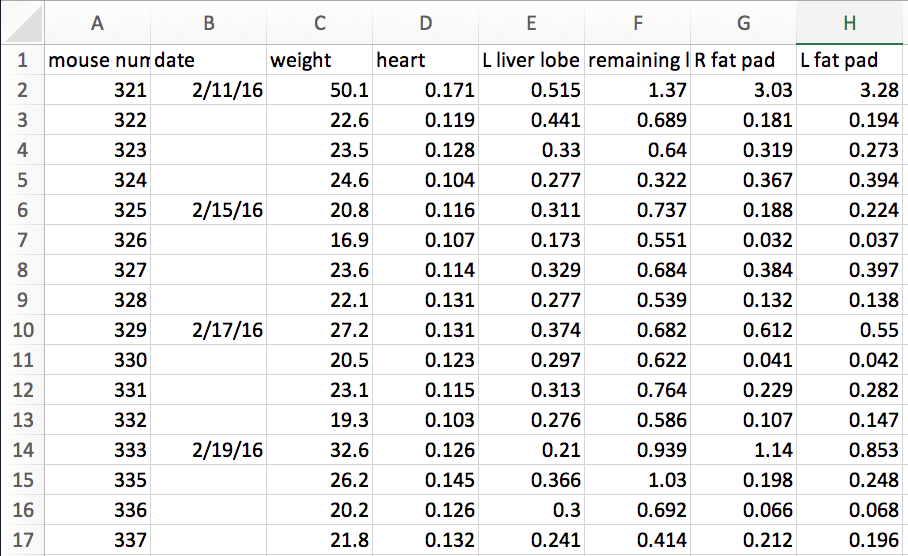
\includegraphics[height=0.6\textheight]{Figs/attiedo_wave4_sacwts.png}
  }

  \only<4>{
    \vspace{-0.5\textheight}
    \hspace{0.3\textwidth}
  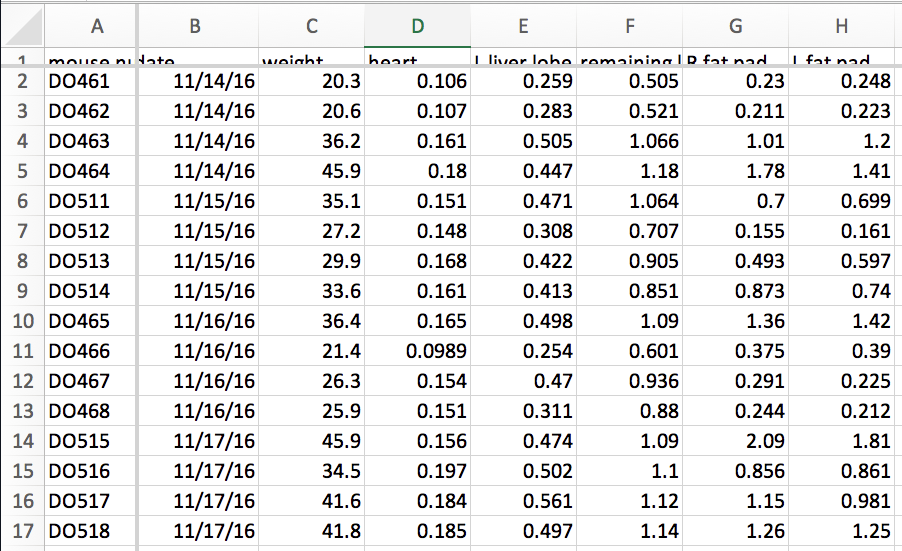
\includegraphics[height=0.6\textheight]{Figs/attiedo_wave5_sacwts.png}
  }

\note{
  The layouts, IDs, and included information are all inconsistent here.
}
\end{frame}




\begin{frame}[c]{Multiple rectangles}

\figw{Figs/attiedo_multicolumn.png}{1.0}

\note{
  Here's an example where they have a group of columns with one set of
  data, a few blank columns, then a group of columns with another set
  of data.
}

\end{frame}







\begin{frame}{Stuff moving around}

  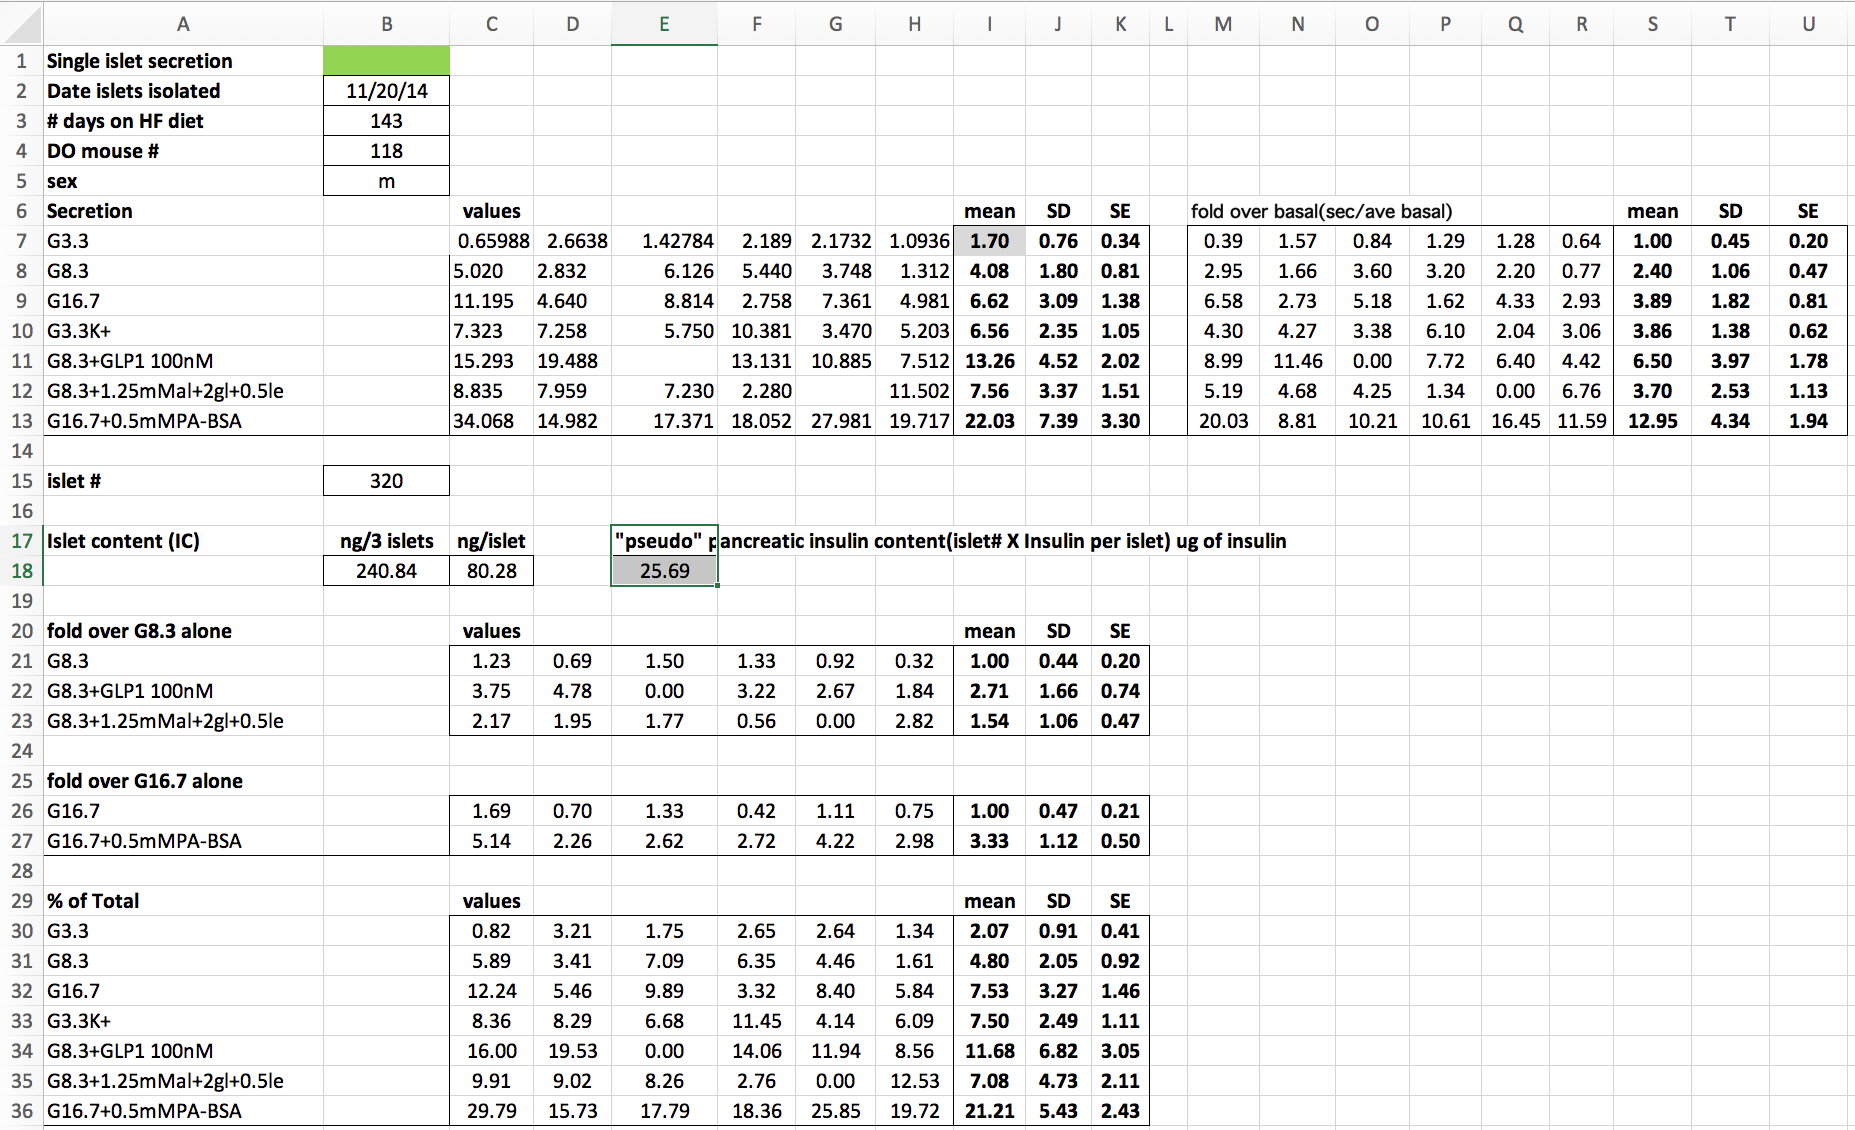
\includegraphics[width=0.8\textwidth]{Figs/attiedo_do118_exvivo.png}

  \only<2>{
    \vspace{-0.65\textheight}
    \hspace{0.1\textwidth}
    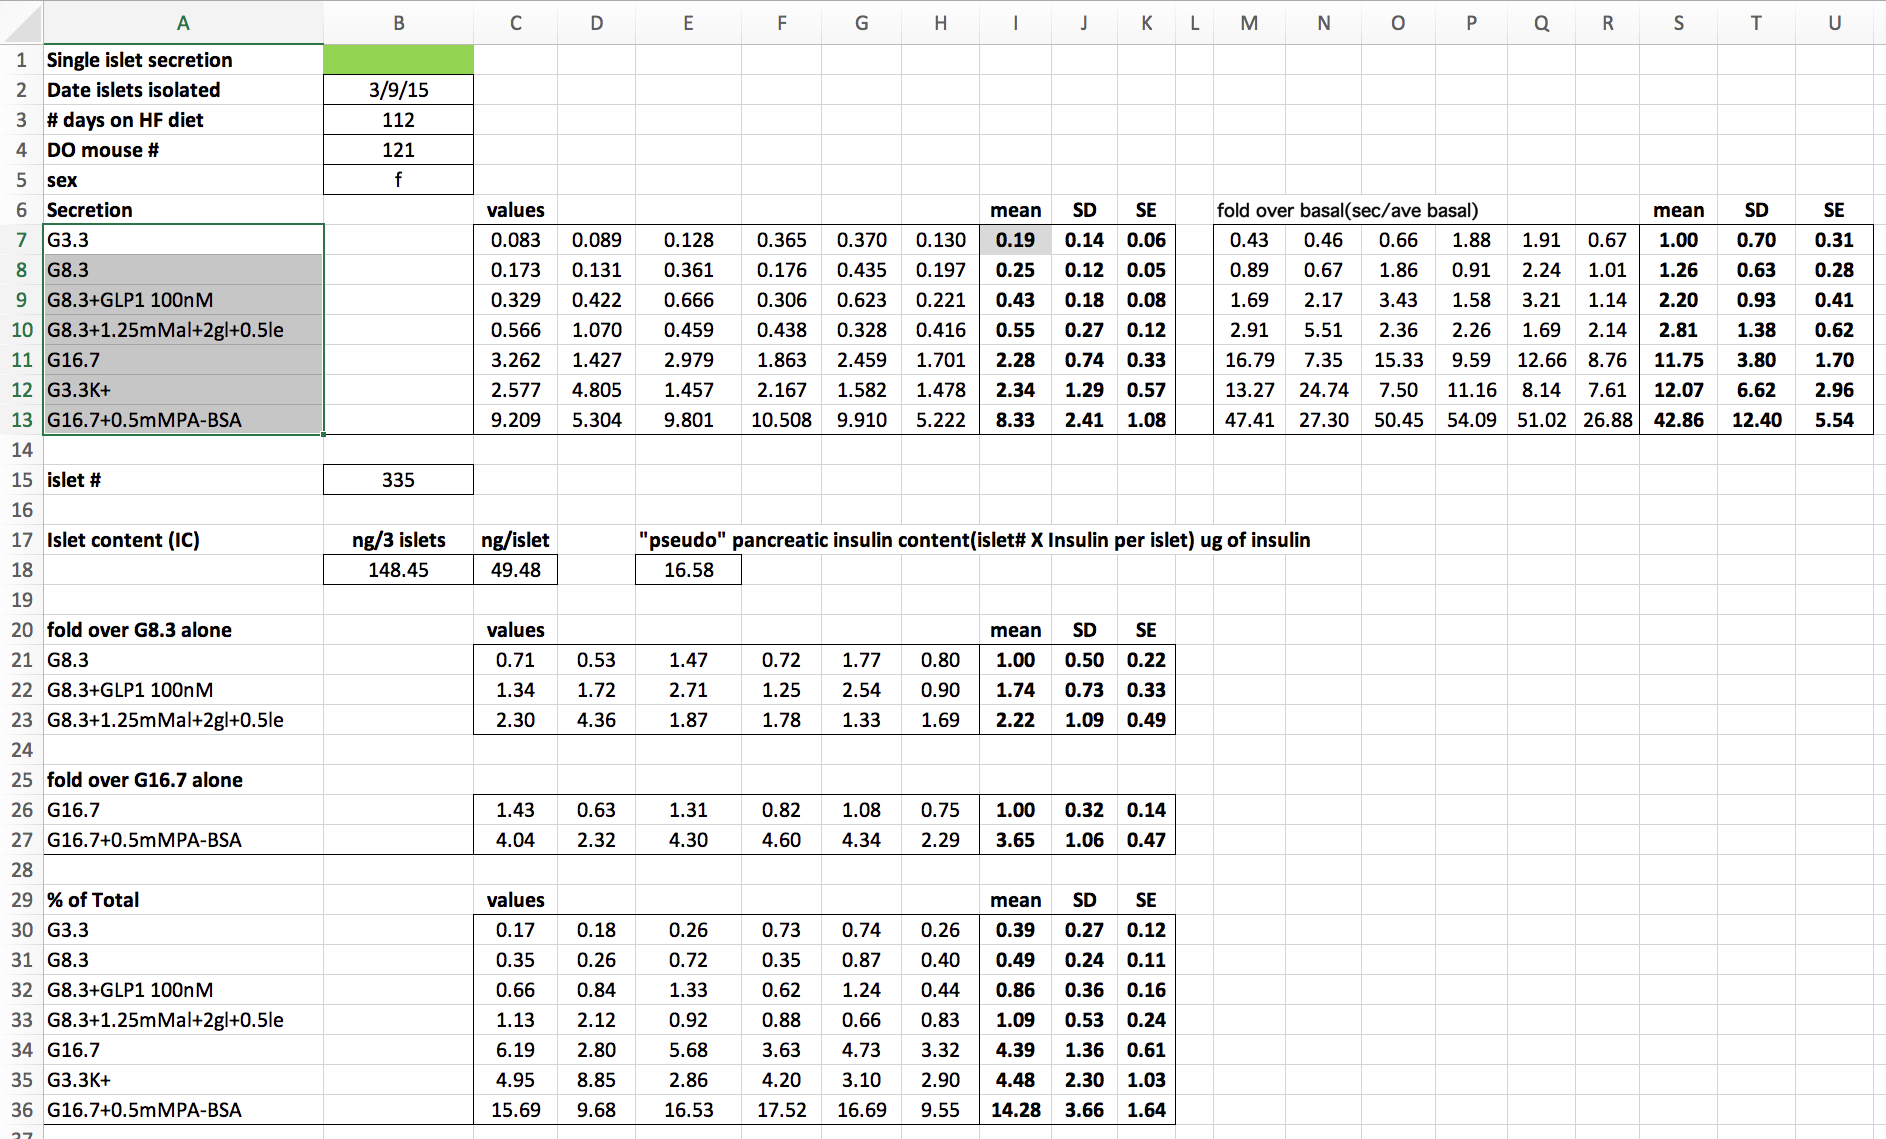
\includegraphics[width=0.8\textwidth]{Figs/attiedo_do121_exvivo.png}
  }


  \note{
    This has a super-complicated layout, has 500 worksheets with one
    mouse each, and the order of things aren't entirely consistent.
  }
\end{frame}



\begin{frame}{Being self-sufficient}

  \bbi
\item {\hilit C}
\item {\hilit P}erl (or python or ruby\only<2>{ or R})
\item {\hilit R}
  \ei

    \note{
      I've long said that for a data scientist to be self-sufficient,
      they should be savvy with multiple programming languages.

      R for data analysis. C for when you need high-performance, and
      for like 15 years I used Perl for manipulating data files plus
      shell scripting.

      But I'd now say use Python or Ruby instead of Perl; probably
      Python. And really, I think we can now do everything we want to
      do in R. It's a perfectly sufficient general programming language.
    }

\end{frame}




\begin{frame}{Key techniques}

  \bbi
\item stepping through a file
\item regular expressions
  \bi
  \item search and replace patterns
  \ei
\item parsing individual lines in a file
\item matching vectors
\item construct meta data
\item system calls
  \ei

\note{
  Here are some of the key techniques that I use to wrangle messy data
  files. I'll go through many of these in more detail.
}


\end{frame}








\begin{frame}[fragile,c]{Stepping through a file in R}

\begin{lstlisting}
  filecon <- file("huge_data.txt", "r")
  while(TRUE) {

    line <- readLines(filecon, n=1)
    if( grepl("^\\[Data\\]", line) )  break

  }

  data <- readLines(filecon)
  close(filecon)
\end{lstlisting}


\note{
  I often use {\tt readLines()} to slurp up an entire file as a vector
  of character strings.

  For really big files, I might want to read one or a few lines at a
  time instead, and throw out all but the stuff that matters. You can
  do this in R!

  This particular example will skip over a header that ends with
  [Data] and then read in everything after that.
}
\end{frame}







\begin{frame}[fragile]{Regular expressions}

  \only<1|handout 0>{\figh{Figs/xkcd_regular_expressions.png}{0.8}

    \vspace{4mm}

    \hfill \href{https://xkcd.com/208}{\tt xkcd.com/208} }
  \only<2|handout 0>{\figh{Figs/regex_cover.jpg}{0.9} }

  \only<3>{
    \bigskip

  {\hilit {\tt grep()}, {\tt grepl()}, {\tt sub()}, {\tt gsub()}}

  \bigskip

  \bi
\item {\tt \textasciicircum} and {\tt \$} match the beginning and end of a line
\item {\tt [034]} for any one of several things; {\tt [0-9]} for a range
\item {\tt [{\textasciicircum}034]} for something {\hilit other} than this set of things
\item {\tt {\textbackslash}s} for white space
\item {\tt .} match any one character
\item {\tt +} match the last bit 1 or more times
\item {\tt *} match the last bit 0 or more times
\item parentheses to group bits for use with {\tt +} and {\tt *}
\item when substituting, can use {\tt {\textbackslash}1}, {\tt {\textbackslash}2}, ... in place of
  matched groups
\item In R, most backslashes need to be made double-backslashes.
\ei
}

\note{
  Regular expression are {\vhilit} hugely useful for the data
  wrangling work.
}
\end{frame}







\begin{frame}{Parsing strings}

  \bbi
\item I use a lot of {\tt strsplit()}
\item The output is a list of vectors so is not pretty
\item Also look at the {\tt stringr} package
\item To put things back together, use {\tt paste()}, {\tt paste0()},
  or the {\tt glue} package.
\ei

\note{
  Messing about with strings is not as easy as in perl, python or
  ruby, but it is more and more do-able.
}
\end{frame}






\begin{frame}{Matching vectors}

  \bbi
\item I spend a lot of time matching two vectors, say of subject IDs
\item I mostly use {\tt match()}, eg {\tt match(old\_ids, new\_ids)}
\item Check for {\tt NA}s, which indicate unmatched values
\item May want to check that the values on right are unique
\item Often do something like {\tt olddata[ match(new\_ids, old\_ids), ]}
\ei

\note{
  Matching IDs is a constant; I mostly use {\tt match()}. Don't assume
  that the values are unique or that they're all present.

  I often use this to reorder the rows or columns in one data set to
  match the rows or columns in another data set.
}
\end{frame}






\begin{frame}[c]{Construct meta data}


\figh{Figs/attiedo_metadata_example.png}{0.9}


\note{
  This is an example meta data file that I set up because each batch
  of subjects in a project had the data organized completely
  differently.

  I identified the variables of interest and chose a fixed set of
  names.

  Then for each batch, I worked out which file it was in, the name of
  the column to look for, and then I also needed a column ``offset''
  because to find week 4 measurements for variable X, you might look
  for the column that is two to the right from the one labeled Y.
}
\end{frame}





\begin{frame}{R challenges}

  \bbi
\item {\tt stringsAsFactors}
\item {\tt check.names} in {\tt read.csv()}
\item dealing with factors
  \bi
\item levels
\item converting to/from strings
  \ei
\item Consider the {\tt forcats} package
  \ei

\note{
  Categorical data is a problem not just for R, but R does have a lot
  of pain points.
}
\end{frame}


\begin{frame}{Further tips}

\bbi
\item Avoid using numeric indices
  \bi
\item refer to data by variable name and individual ID
\item this will be more {\hilit robust}
  \ei
\item {\tt stopifnot()} to assert things that should be true
\item {\tt cbind} and {\tt rbind}, but padding with missing values
\item Sometimes converting excel $\rightarrow$ csv loses precision
\item {\tt get()} to grab an object from a character string with its
  name
\item {\tt eval(parse( ))} to evaluate a character string as R code
  \ei

  \note{
    Here are some misc.\ further tips.
  }
\end{frame}




\begin{frame}{Verify everything}

\bbi
\item subject IDs unique?
\item identifiers that don't match the typical pattern?
\item subjects in one file but not in another?
\item re-calculate and verify any derived values (like ratios)
\item data repeated in multiple files the same?
\ei

  \note{
    You really should verify everything. Don't trust that things
    match; everything that can go wrong, will.
  }
\end{frame}




\begin{frame}{Reproducible reports}

\bbi
\item You want all of this work to be reproducible
\item Consider combining the data reorganization with the data
  cleaning
  \bi
    \item a lot of double-checking is happening when reorganizing
  \ei
\item Or clean each file one at a time
  \bi
    \item do the detailed diagnostics and cross-checks with data that are
      in a more convenient form
  \ei
\item Include diagnostic plots
  \bi
    \item Plot stuff vs time or by batch
    \item Scatterplots of different variables
    \item Consider taking logs
    \item Look at missing data pattern
  \ei
\item Explain your thought process and observations
  \ei

  \note{
    It is critical that the data re-formatting process be
    reproducible. You are {\hilit very} likely to be doing it more
    than once.

    You often are doing data diagnostics and reformatting
    at the same time.
    Maybe have one long R Markdown or Jupyter
    document that does both? Or maybe it's best to rearrange each
    file, one at a time, and then do the serious diagnostics after
    you've gotten it all into a simpler form.

    For diagnostics, you want to plot each variable against time, or
    by bath. And make scatterplots of different variables. The missing
    data pattern is also often quite informative about problems.
  }
\end{frame}



\begin{frame}[c]{Batch effect}

\only<1|handout 0>{\figh{Figs/il3.pdf}{0.85}}
\only<2>{\figh{Figs/il3_log.pdf}{0.85}}

\note{
Here's an example of a clear batch effect. You can really only tell if
you plot the variable by the order of measurement, and it's much more
clear if you take logs.
}

\end{frame}





\begin{frame}[c]{Messed up units}

\figh{Figs/adipose_weight.pdf}{0.85}

\note{
Here's a case where a variable was recorded in the wrong units (g
rather than mg) for a few individuals)

}

\end{frame}




\begin{frame}[c]{Outliers}

\figh{Figs/body_weight.pdf}{0.85}

\note{
In this particular case, it turned out that the day 10 weights for two
subjects got swapped.

When you look at this sort of situation, ask yourself how you might
find this problem if you have 20 weight measurements and 1500
individuals.
}

\end{frame}




\begin{frame}[c]{Summary}

  \bbi
\item Be prepared for anything
\item Double-check everything
\item Take your time and keep things organized
\item Python is a good skill to have, but you {\vhilit can} just do R
  \ei

\note{
  Summaries are always helpful.
}

\end{frame}



\end{document}
